\documentclass[12pt,a4paper,fontset=none]{ctexart}
\setCJKmainfont{Songti SC}
\setCJKsansfont{Heiti SC}
\setCJKmonofont{Heiti SC}
\usepackage[top=2.54cm,bottom=2.54cm,left=3.17cm,right=3.17cm]{geometry}
\usepackage{setspace}
\onehalfspacing
\setlength{\parindent}{2em}
\usepackage{amsmath,amssymb,booktabs,graphicx,xcolor}
\usepackage[colorlinks=true,linkcolor=black,citecolor=black,urlcolor=black]{hyperref}
\usepackage{caption}
\captionsetup{font=small,labelfont=bf,skip=6pt}
\graphicspath{{figures/}}

\title{肠化生上皮仍落在胃炎范围内：\\公开单细胞图谱上的可加虚拟敲除}
\author{}
\date{}
\begin{document}
\maketitle

\begin{abstract}
\noindent\textbf{目的}\quad 在患者水平上检验：把单个基因的上皮表达置零之后，肠化生是否因此离开胃炎、靠近胃癌。

\noindent\textbf{方法}\quad 使用 GSE249874 的 18 例胃组织单细胞（非萎缩性胃炎、肠化生、胃癌各 6 例）。上皮细胞经基因评分划定后，按患者取对数表达均值。轴由胃癌均值减胃炎均值得到，肠化生不参与定轴。虚拟敲除是可加投影：该基因的位移等于其权重与肠化生表达的乘积，再除以轴长。对照为 12 例胃炎与胃癌标签的 200 次打乱（种子 20261003）。保留要求置换 \(p\le 0.05\)，且 6 次留一中至少 5 次仍高于对应空分布的第 95 百分位。

\noindent\textbf{结果}\quad 质控后 101\,970 个细胞，上皮 19\,649 个。位置中位数为胃炎 10.26、肠化生 11.90、胃癌 18.03。6 例胃癌均高于 6 例胃炎；6 例肠化生的位置在 9.08--12.51，全部落在胃炎范围内。4\,781 个基因进入敲除检验，416 个被保留。保留基因位移中位数的中位为 0.0018，最大为 HSP90AA1 的 0.24。胃炎到胃癌的中位数差为 7.77。CLDN18、HNF4G、CDX2、MUC2 均未保留。

\noindent\textbf{结论}\quad 在这 18 例患者中，肠化生上皮没有进入胃癌区间。单基因置零产生的位移远小于胃炎与胃癌的差距，不能据此指定一个把肠化生推回或推向胃癌的基因。
\end{abstract}

\textbf{关键词：}胃癌；肠化生；单细胞转录组；虚拟敲除

\vspace{0.6em}
\noindent\textbf{Abstract.} On the public single-cell atlas GSE249874 (6 non-atrophic gastritis, 6 intestinal metaplasia, 6 gastric cancer), an epithelial axis was the difference between cancer and gastritis patient means. Metaplasia was not used to fit the axis. Setting one gene to zero changed a patient's position by that gene's weight times its metaplasia expression, divided by the length of the axis. Median positions were 10.26, 11.90 and 18.03. All six metaplasia samples lay inside the gastritis range. Of 4\,781 tested genes, 416 passed the pre-specified permutation and leave-one-out rule, but their median displacement was 0.0018 and the largest, HSP90AA1, was 0.24, against a gastritis-to-cancer gap of 7.77. CLDN18, HNF4G, CDX2 and MUC2 were not retained.

\section{引言}

Li 等对 18 例胃黏膜做了单细胞测序，标本按病理分为非萎缩性胃炎、肠化生和胃癌，每组 6 例，并记录幽门螺杆菌状态\cite{li2025}。该文描述了上皮、成纤维和髓系细胞在这一过程中的组成，并把 HNF4G 作为肠化生肠上皮细胞的转录因子候选。

本稿不重复那张细胞图谱。问题改成患者水平的上皮状态：胃炎和胃癌的上皮均值能否拉开；肠化生落在哪一侧；把一个基因置零之后，肠化生的位置移动多少。移动量按可加投影计算。它等于该基因在轴上的贡献，不是细胞状态的动力学轨迹，也不是药物作用。

\section{资料与方法}

\subsection{数据与质控}

计数矩阵取自 GEO 系列 GSE249874，平台为 10x Genomics 3' v3.1，参考基因组 hg38\cite{li2025}。18 个文库按样本顺序各占连续的 6\,794\,880 个白名单条码。有计数的条码共 19\,688\,657 个。白名单中的空条码不进入后续计算。

质控阈值沿用原论文写出的数字：基因数不少于 200，UMI 不少于 1\,000，\(\log_{10}\)（基因数）/\(\log_{10}\)（UMI）不低于 0.7，线粒体比例不高于 20\%，血红蛋白基因比例不高于 5\%。原论文另用 DoubletFinder 去除双细胞，本稿没有这一步。表达在每个细胞上归一到 1 万后再取 \(\log(1+x)\)。

\subsection{上皮与患者向量}

上皮评分基因为 EPCAM、KRT8、KRT18、KRT19，免疫为 PTPRC、CD3D、CD79A、MS4A1，成纤维为 COL1A1、DCN、LUM。细胞需上皮评分大于 0，且高于免疫评分和成纤维评分。患者上皮细胞少于 50 个则不进入轴和敲除。上述 11 个基因以及线粒体、血红蛋白基因不进入敲除名单。每个患者的向量是其上皮细胞对数表达的均值。统计单位是患者。

\subsection{轴与虚拟敲除}

轴只用 6 例胃炎和 6 例胃癌。基因权重是胃癌均值减去胃炎均值。进入轴的基因，须在至少 4 例胃炎和 4 例胃癌中，上皮检出比例都不低于 10\%。患者位置是该向量与权重的点积除以权重长度。位置越高，越靠胃癌一端。肠化生不参与定轴。

对权重大于 0 的基因做置零。一个患者的位移等于该基因权重乘以其上皮均值，再除以轴长。基因还须在至少 4 例肠化生中达到 10\% 检出。对照把 12 例胃炎和胃癌的标签打乱 200 次，种子 20261003，肠化生的表达不变。置换 \(p=(1+\)空分布中不小于观察值的次数\()/201\)。

保留同时满足两条：6 例肠化生位移中位数的置换 \(p\le 0.05\)；每次去掉 1 例肠化生后，其余 5 例的中位数仍高于这 5 例自身空分布的第 95 百分位，6 次里至少 5 次成立。幽门螺杆菌不参与这条规则。CLDN18、HNF4G、CDX2、MUC2 事先点名，不因结果改阈值。

\section{结果}

\subsection{上皮轴把胃癌和胃炎分开，肠化生留在胃炎一侧}

质控由 145\,186 个达到基因数、UMI 和比值门槛的细胞减到 101\,970 个。上皮细胞 19\,649 个，18 例患者都不少于 50 个。最少的是肠化生 GSM7966238，100 个上皮细胞。

位置中位数为胃炎 10.26、肠化生 11.90、胃癌 18.03（图~\ref{fig:position}）。6 例胃癌的最低值为 16.06，6 例胃炎的最高值为 15.52，两组没有重叠。6 例肠化生位于 9.08--12.51，全部落在胃炎的最小值和最大值之间，没有一例进入胃癌区间。肠化生的中位数高于胃炎中位数，但患者个体仍在胃炎范围内。

\begin{figure}[htbp]
  \centering
  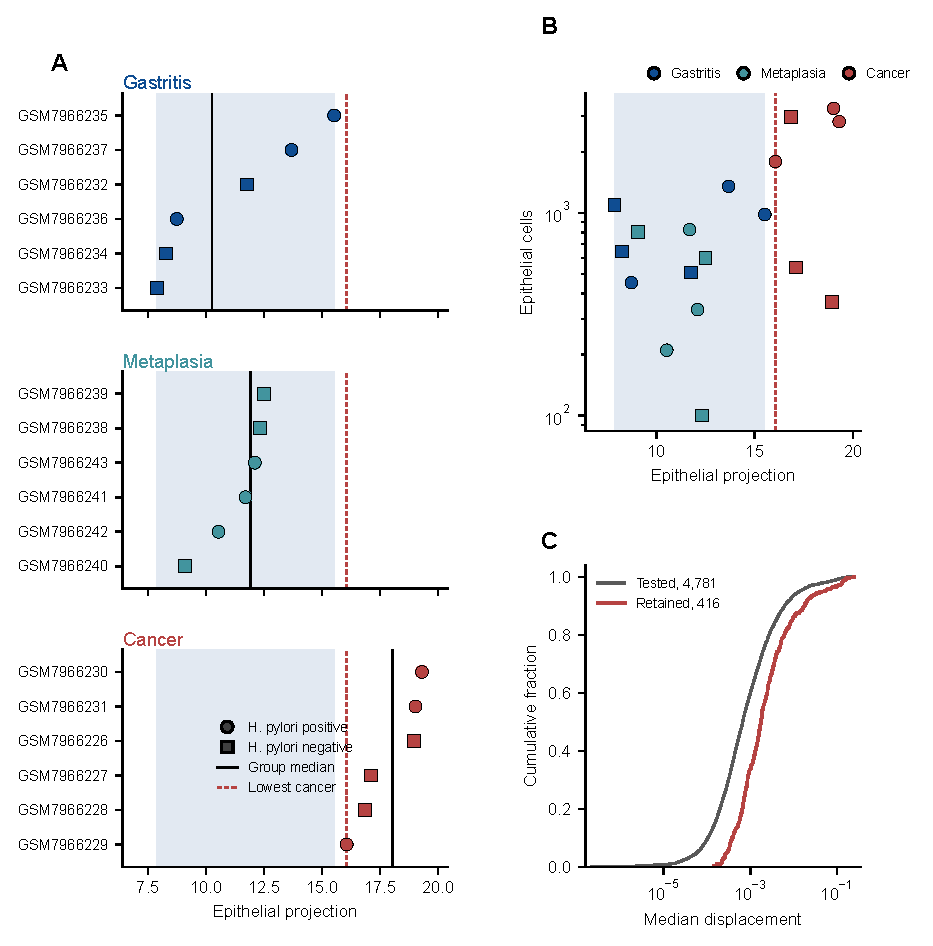
\includegraphics[width=0.78\textwidth]{fig_position.pdf}
  \caption{18 例患者的上皮投影。点为患者，短横线为该组中位数。纵轴是对数表达均值在胃炎--胃癌轴上的投影，轴由两组均值之差定义，肠化生未参与定轴。}
  \label{fig:position}
\end{figure}

\subsection{单基因位移远小于组间差距}

轴上有 7\,411 个基因。其中权重为正、且在肠化生达到检出要求的有 4\,781 个。416 个同时通过置换和留一。这 416 个位移的中位是 0.0018，最大是 HSP90AA1 的 0.24。胃炎与胃癌的中位数差为 7.77。图~\ref{fig:ko} 把位移最大的 12 个基因和这条差距放在同一标尺上。前 12 位里，除 HSP90AA1、HSP90AB1 外，其余是核糖体蛋白（表~\ref{tab:top}）。

\begin{figure}[htbp]
  \centering
  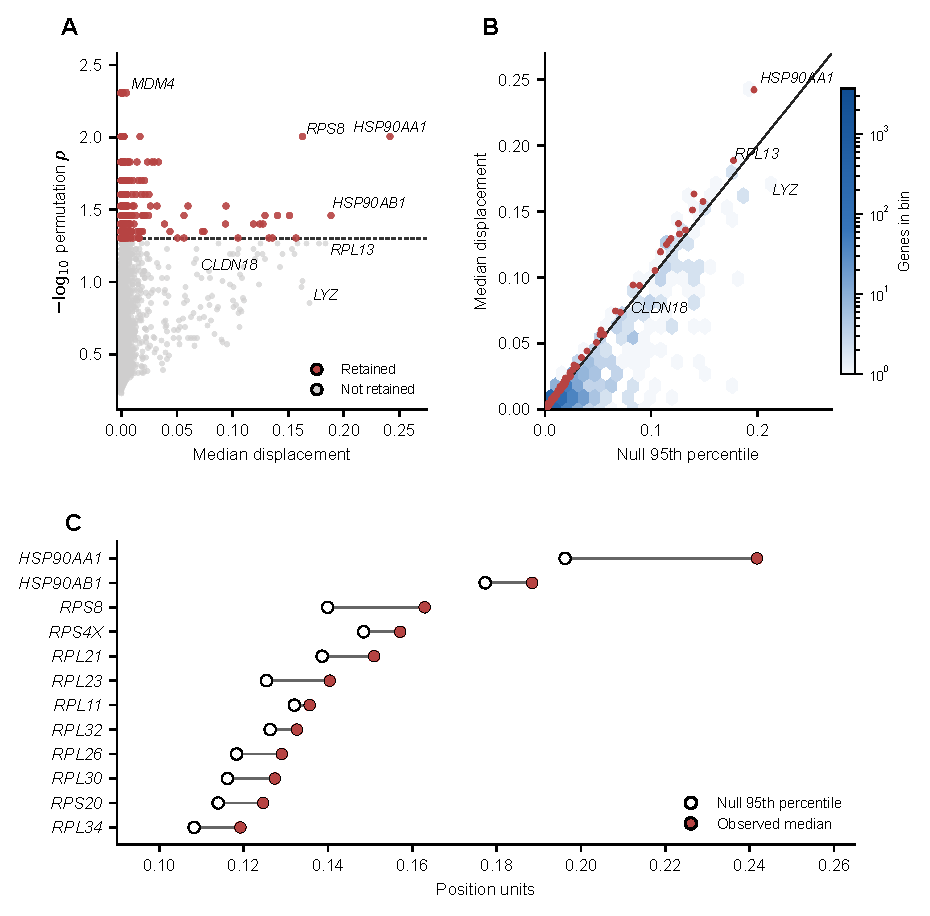
\includegraphics[width=0.86\textwidth]{fig_knockout.pdf}
  \caption{左：416 个保留基因里位移最大的 12 个，横轴放到 0.30，以便看出高低。右：同一单位下，HSP90AA1 的 0.24 与胃炎--胃癌中位数差 7.77。柱没有误差线，因为报告的是 6 例肠化生的中位数，没有另估标准误。}
  \label{fig:ko}
\end{figure}

\begin{table}[htbp]
  \centering
  \caption{位移最大的 12 个保留基因。置换 \(p\) 的分母为 201。留一列为 6 次中通过的次数。}
  \label{tab:top}
  \small
  \begin{tabular}{lrrr}
    \toprule
    基因 & 肠化生位移中位数 & 置换 \(p\) & 留一 \\
    \midrule
    HSP90AA1 & 0.242 & 0.010 & 6 \\
    HSP90AB1 & 0.188 & 0.035 & 6 \\
    RPS8     & 0.163 & 0.010 & 6 \\
    RPS4X    & 0.157 & 0.050 & 6 \\
    RPL21    & 0.151 & 0.035 & 6 \\
    RPL23    & 0.140 & 0.035 & 6 \\
    RPL11    & 0.136 & 0.050 & 6 \\
    RPL32    & 0.133 & 0.050 & 6 \\
    RPL26    & 0.129 & 0.035 & 6 \\
    RPL30    & 0.127 & 0.040 & 6 \\
    RPS20    & 0.125 & 0.040 & 6 \\
    RPL34    & 0.119 & 0.040 & 6 \\
    \bottomrule
  \end{tabular}
\end{table}

事先点名的四个基因都没有保留（表~\ref{tab:pre}）。CLDN18 权值为正，位移 0.068，置换 \(p=0.090\)，留一 0 次。HNF4G 权值为负，胃炎端更高，位移为 \(-0.002\)。CDX2 和 MUC2 未进入轴，因为它们不满足至少 4 例胃炎和 4 例胃癌都达到 10\% 检出。

\begin{table}[htbp]
  \centering
  \caption{事先点名的基因。空缺表示该基因未进入轴。}
  \label{tab:pre}
  \small
  \begin{tabular}{lrrrl}
    \toprule
    基因 & 权重 & 位移中位数 & 置换 \(p\) & 结果 \\
    \midrule
    CLDN18 & 0.673 & 0.068 & 0.090 & 未保留 \\
    HNF4G  & $-0.142$ & $-0.002$ & 0.985 & 未保留 \\
    CDX2   & --- & --- & --- & 未入轴 \\
    MUC2   & --- & --- & --- & 未入轴 \\
    \bottomrule
  \end{tabular}
\end{table}

\section{讨论}

这 18 例里，胃癌上皮和胃炎上皮在投影上分开，肠化生的 6 个患者仍落在胃炎的范围内。中位数的次序是胃炎、肠化生、胃癌，但这个次序没有把肠化生患者移出胃炎区间。用“中位数位于两组之间”描述这组肠化生，会高估它向胃癌的移动。

416 个基因通过了事先写定的保留线。通过的原因主要是空分布也很窄，不是位移已经接近组间差距。最大位移 0.24，约为差距 7.77 的 3\%。排在前面的热休克蛋白和核糖体蛋白，对应的是胃癌上皮相对胃炎上皮的一批高表达基因，不是一个可以单独置零就改变患者位置的节点。

HNF4G 在原图谱里被标为肠化生肠上皮的转录因子候选\cite{li2025}。在本稿的患者轴上，它的权重为负，且没有通过保留线。两句判断用的不是同一套汇总：原文献看的是肠化生内部的细胞亚群，本稿看的是胃炎对胃癌的患者均值。CDX2 和 MUC2 未入轴，只说明它们没有在两端都达到预设检出，不能据此写成这两个基因在肠化生里没有表达。

幽门螺杆菌状态按组各有 3 例，本稿没有把它放进主检验。上皮细胞数在患者之间差得很大，GSM7966238 只有 100 个上皮细胞，这个患者的均值更不稳定。可加投影也不描述基因之间的代偿：置零一个基因时，其余基因表达保持原值。

\section{结论}

GSE249874 的上皮投影把 6 例胃癌和 6 例胃炎分开。6 例肠化生都留在胃炎的位置范围内。在预设规则下，416 个基因的单基因位移远小于 7.77 的组间中位数差。CLDN18、HNF4G、CDX2 和 MUC2 都没有成为保留基因。

\section*{数据与代码}

GSE249874 的计数矩阵可从 GEO 获取。本稿使用的患者位置表和基因敲除表由该矩阵按第 2 节的规则计算，随分析记录保存。脚本尚未存入公共代码库。

\begin{thebibliography}{9}
\bibitem{li2025}
Li N, Chen S, Xu X, Wang H, Zheng P, Fei X, et al.
Single-cell transcriptomic profiling uncovers cellular complexity and microenvironment in gastric tumorigenesis associated with \textit{Helicobacter pylori}.
\textit{J Adv Res}. 2025;74:471--491.
doi:10.1016/j.jare.2024.10.012.
\end{thebibliography}

\end{document}
